\documentclass[twoside]{article}

\usepackage[utf8]{inputenc}
\usepackage{comment}
\usepackage{todonotes}
\usepackage{msc5}
\usepackage{listings}
\usepackage{url}
\usepackage{tikz-qtree}

\usepackage{amsmath, amssymb, amsthm, amsfonts, caption, stmaryrd, mathtools, syntax, mdframed}

\newenvironment{prog}{\begin{array}[t]{@{}l@{}}}{\end{array}}

\newcommand{\adv}{{\sf Adv}}
\newcommand{\madv}{\mathsf{Adv}}
\newcommand{\CSess}{\mathcal{C}}
\newcommand{\SSess}{\mathcal{S}}
\newcommand{\laction}[2]{$\begin{array}{c}\mbox{\textrm{#1}}\\#2\end{array}$}
\newcommand{\Z}{\mathbb{Z}}
\newcommand{\Zp}{\mathbb{Z}_p}
\newcommand{\M}{\mathbb{M}}
\newcommand{\SIGN}{\mathsf{SIGN}}
\newcommand{\HMAC}{\mathsf{HMAC}}
\newcommand{\HKDF}{\mathsf{HKDF}}
\newcommand{\ENC}{\mathsf{ENC}}
\newcommand{\DEC}{\mathsf{DEC}}
\newcommand{\sk}[1]{\mathit{sk}_{#1}}
\newcommand{\vk}[1]{\mathit{vk}_{#1}}
\newcommand{\shared}{\mathit{shared}}
\newcommand{\const}{\mathit{const}}
\newcommand{\e}{\mathit{enc}}
\newcommand{\m}{\mathit{mac}}
\newcommand{\rk}{\mathit{rk}}
\newcommand{\ck}{\mathit{ck}}
\newcommand{\tg}{\mathit{tag}}
\def\hash#1{\mathsf{H}(#1)}
\def\sign#1#2{\mathsf{sign}^{#2}(#1)}
\def\hmac#1#2{\mathsf{HMAC\mbox{-}H}^{#2}(#1)}
\def\mac#1#2{\mathsf{mac}^{#2}(#1)}
\def\tlsmac#1#2{\mathsf{mac}_{96}(#2,#1)}
\def\aead#1#2#3{\mathsf{aead}^{#2}(#1)}
\def\aenc#1#2{\mathsf{enc}^{#2}(#1)}
\def\adec#1#2{\mathsf{dec}^{#2}(#1)}
\def\mac#1#2{\mathsf{mac}^{#2}(#1)}
\def\kdf#1{\mathsf{kdf}(#1)}
\def\kdfcontext#1#2{\mathsf{kdf}(#1,#2)}
\def\dh#1#2{\mathsf{dh}(#1,#2)}
\def\kdfi#1#2{\mathsf{kdf}_{#1}(#2)}
\def\kdfz{\mathsf{kdf}_0}
\def\hkdf#1{\mathsf{hkdf}(#1)}
\def\dlog#1{\mathsf{dlog}(#1)}
\def\factor#1{\mathsf{factor}(#1)}
\def\cert{\mathit{cert}}
\def\kex{\mathit{kex}}
\def\pk{\mathit{pk}}
\def\sk{\mathit{sk}}
\def\pkp#1{\mathit{pk}_#1}
\def\skp#1{\mathit{sk}_#1}
\def\vd#1#2{\mathsf{finished}(#2,#1)}
\def\anon{\mathtt{anon}}
\def\pms{\mathit{pms}}
\def\keys{\mathit{keys}}
\def\log{\mathit{log}}
\def\ctx{\mathit{ctx}}
\def\ms{\mathit{ms}}
\def\cvd{\mathit{cvd}}
\def\svd{\mathit{svd}}
\def\sid{\mathit{sid}}
\def\mod{\mathbin{\mathrm{mod}}}
\def\info{\mathit{info}}
\def\cfg{\mathit{cfg}}
\def\nego{\mathit{nego}}
\def\uid{\mathit{uid}}
\def\pref{\mathit{Nego}}
\def\cid{\mathit{cid}}
\def\ems{\mathit{ems}}
\def\psk{\mathit{psk}}
\def\ctx{\mathit{ctx}}
\def\hk{\mathit{hk}}
\def\dk{\mathit{dk}}
\def\ak{\mathit{ak}}
\def\sni{\mathit{sni}}
\def\dsni{d_\mathit{sni}}

\theoremstyle{definition}
\newtheorem{definition}{Definition}[section]

\title{Encrypted SNI: Privacy and Security}
\author{No Name}
\date{\today}

\begin{document}

\maketitle

\begin{comment}
# Outline
- ESNI use cases, overview, and desired security goals:
    - Use cases:
        - Name privacy (coupled with DNS) against "active" attacker (modulo traffic analysis), local service discovery
    - Operational requirements and criteria: (listed from the draft)
    - Design overview:
        - Summary of draft 4
        - Overview of related designs
    - Four security/privacy requirements:
        - ESNI privacy (requirement #2):
            1. Both endpoints agree on the context
            2. Agreement implies knowledge of SNI and key share
            3. Client has proof that server has private ESNI key
    - Passive attacker: 
        - Probabilistic public key encryption (is sufficient?)
    - Known active attacks and observations:
        - Probing (client offline, draft 4): Differences in service configurations can leak information.
        - HRR mix and match (client offline, draft 4): Attacker-chosen key share, client-chosen SNI.
        - Server reaction attack (client offline, draft 4): Use ticket and server reaction for dictionary attack.
        - Client reaction attacks (earlier draft, client online): Include nonce so that same entity which sent certificate actually processed the ESNI value.
        <!-- - HRR trial decryption (client offline): Client-chosen SNI, server-chosen key share. -->
        <!-- - PSK and ENSI (draft 4): Change CH ESNI value to be attacker-controlled, and server aborts or not based on SNI+PSK equality -->
- Basic anonymous DH model (handshake secret integrity):
    - (Challenge response with the nonce)
    - Two messages (CH, SH), and proof
    - Four messages (CH1, HRR, CH2, SH), and proof
- Handshake side channels
    - (Data about handshake message size distribution?)
    - (Application data side channels -- defer to future work?)
    - CH and SH generation functions and requirements
- Integration with TLS
    - Proxy-based transformation
    - PSK binder and key schedule injection
    - (Signalling via SH.Random or explicit SH extension)
- Implementation and experimentation
\end{comment}

\begin{comment}
# Notes
- Assume that application data transfer leaks nothing about the service.

bindings: cast in terms of contexts (transcripts)
Backward binding: integrity for ClientHello
Forward binding: 
- want to detect deletion of SNI
- proxy needs DH secrets to determine the right transcript -- can't be two entities on the client side
- could treat origin padding as a configuration
- GeneraetSH must be done at the proxy, and not based on origin servers. Can get away with unmodified servers (modulo template)
- GeneraetCH/SH are the baseline properties -- show that adding forward/backward binding keeps existing properties while giving new properties
  - These may be determined by checkboxes. If any two F's are the same, then the privacy properties hold.
  - Q: should ACME be issuing certificates of a certain length

- flipping bits in CH should cause handshake keys to differ (Kazuho's does NOT do this, and there's an oracle at the client handshake)
- always need backwards binding (for messages, but possibly based on the entire transcript?)
- kazuho: enumerate domains and trial decrypt based on all possible transcripts

What we want to hide:
- SNI value itself
- A connection negotiated ESNI
- Whether the ESNI capability
- Whether the client offered ESNI

Requirements:
1. TLS agrees on SNI (forward binding, native to TLS)
2. TLS+ESNI gives us (1) and protects SNI privacy (backward binding)
  - 1/k anonymity, without forward secrecy

Optional:
3. TLS+ESNI gives (1-2) and protects the fact that ESNI was chosen
4. TLS+ESNI (1-3), plus whether the client offered ESNI


%%% Agenda:
%** Writeup review
%** ProVerif basic model with attacks -- should the ServerHello have a signal?
%** Writeup of how Kazuho/Steven PRs satisfy the basic model
%** Game-based definition (port)
\end{comment}

\section{Introduction}

\todo[inline]{writeme}

\section{Encrypted SNI}

%% XXX: outline use cases
%% XXX: misconfigurations where use of public name goes to a server that does not negotiate ESNI but does offer a certificate that terminates to the public name
%% XXX: draw figures of deployment scenarios

There are several operational goals for Encrypted SNI \cite{requirements}, described below:
%
\begin{itemize}
  \item Work with non-ESNI servers to avoid fallback.
  \item Mitigate replay attacks:
  \item Avoid widely-deployed shared secrets: 
  \item Prevent SNI-based DoS attacks:
  \item Do not stick out:
  \item Forward secrecy:
  \item Proper security context:
  \item Split server spoofing:
  \item Multiple protocol support:
\end{itemize}
%

\subsection{Draft-04 Design Overview}
XXX: include figure of the protocol

\subsection{Security and Privacy Goals}
ESNI assumes a standard active and on-path Dolev-Yao attacker that can arbitrarily drop, tamper, 
replay, and forward messages from clients. Fundamentally, a TLS handshake that negotiates ESNI should 
leak no more information than one which did not negotiate ESNI in the presence of this adversary. 
This means there are at least two necessary requirements for ESNI:
%
\begin{enumerate}
  \item SNI agreement: A successful TLS handshake implies agreement on the SNI transmitted. This means, among 
  other things, that the client authenticated the server's certificate using the SNI, and that both client and 
  server share the same view of the SNI negotiated.
  \item SNI privacy: A successful TLS handshake that negotiates ESNI does so without leaking any information 
  about the underlying SNI. Moreover, the SNI is known only to the client and server (or any recipient of the
  private ESNI key). We do not require forward secrecy for the SNI encryption.
\end{enumerate}
%
We may optionally want to hide the fact that ESNI was negotiated, as per the ``do not stick out'' goal. However, 
this is primarily only deployment concern. Furthermore, we may also want to hide the fact that a client offered
ESNI in its handshake. This may be useful for clients that wish to GREASE \cite{XXX} the extension.

\subsection{Known Attacks} \label{sec:known-attacks}

Early versions of ESNI did not achieve these goals. For example, the first version was vulnerable to a certificate-based 
client reaction attack shown in Figure \ref{fig:attack1-client-reaction}. The core problem was that servers did not signal
to clients whether or not they processed the ESNI extension. This allowed any MITM to complete the handshake
-- prior to authentication -- on behalf of the server with a certificate of its choosing. Adding a nonce to the server's
response prohibits this as clients can then check whether or not the nonce is correct.

% XXX: rewrite me using msc as below
\begin{figure}
    \centering
    % 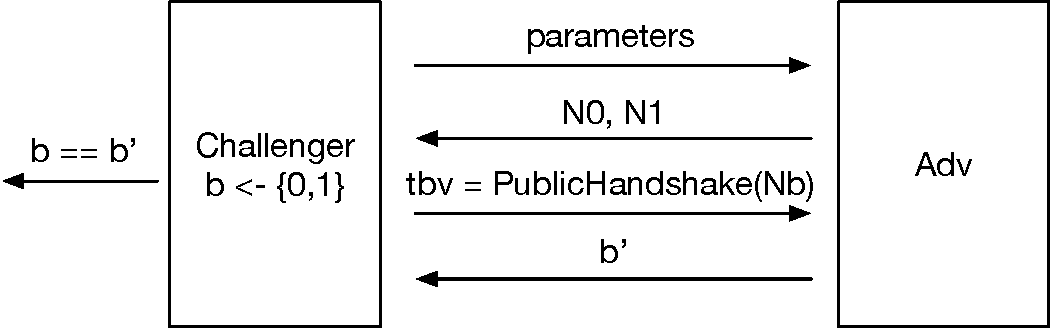
\includegraphics[scale=0.7]{esni_game.pdf}
    \caption{Early ESNI Client Reaction Attack}
    \label{fig:attack1-client-reaction}
\end{figure}

Despite this fix, draft-04 of ESNI does not achieve the necessary requirements stated above. To show why, we 
illustrate some more attacks on the protocol.

\begin{description}
  \item[Probing Attacks]: Differences in service configurations can leak information.
  \item[HelloRetryRequest Mix and Match]: Attacker-chosen key share, client-chosen SNI.
  \item[Server Reaction Attacks]: Use ticket and server reaction for dictionary attack.
\end{description}

The number of edge cases makes it clear that a formal model of the protocol is needed.

\section{Core Protocol} % Basic anonymous DH model (handshake secret integrity)

At its core, ESNI is a protocol between a client and server that works as described in
Figure \ref{fig:simple-esni}. It aims to provide the following guarantees:
%
\begin{itemize}
  \item Client: TLS handshake secret known by entity which has the private handshake key share (y), corresponding PSK,
  private ESNI decryption key, and ENSI nonce. 
  \item Server: TLS handshake secret known by entity which has the private handshake key share (x), corresponding PSK,
  and ENSI nonce.
  \item Client and server both agree on the same TLS handshake secret and transcript.
\end{itemize}
%

\def\offer{\mathit{offer}}
\def\mode{\mathit{mode}}

\begin{figure}[th!]
%\begin{minipage}{\columnwidth}
\begin{center}
\resizebox{0.8\columnwidth}{!}{\begin{msc}{}
  \drawframe{none}
  \setlength{\topheaddist}{0cm}
  \setlength{\instdist}{8.5cm}
  \setlength{\instwidth}{1.75cm}
  \declinst{cl}{}{Client $C$}
  \declinst{sr}{}{Server $S$}
  \action*{$\mathit{Knows}\ \sni, \psk$}{cl}
  \action*{$\mathit{Knows}\ \dsni, (\skp{S},\pkp{S}), \psk$}{sr}
  \nextlevel[2]
  \nextlevel
  \mess{\emph{Client Flight} ($S, g^x, \mathsf{Enc}(K_s, (r, \sni))$)}{cl}{sr}
  \nextlevel[2]
  \action*{\laction{Derive ESNI Keys:}{
    ss = \dh{g^y}{g^x} \\
    k = \kdfcontext{ss}{"esni"}}}{sr}
  \nextlevel[5]
  \mess{\emph{Server Flight} ($g^y,\mathsf{enc}(k, r)$)}{sr}{cl}
  \nextlevel
  \action*{\laction{Derive ESNI Keys:}{
    ss = \dh{g^x}{g^y} \\
    k = \kdfcontext{ss}{"esni"}}}{cl}
  \nextlevel[3]
  \end{msc}
}
\end{center}
\caption{Simple ESNI Protocol without resumption or HelloRetryRequest support.}
\label{fig:tls-structure}
\end{figure}

Moreover, these guarantees must hold for all TLS handshake patterns, including: normal handshakes,
resumption handshakes, and HelloRetryRequest handshakes. Considering the full variant, there are 
five secrets that influence the handshake: private signing key, secret Diffie Hellman key shares,
pre-shared key(s), ESNI decryption key ($K_S$), and the ESNI nonce. Informally, we require that
these values endorse each other in order to avoid the attacks described in Section \ref{sec:known-attacks}.

XXX: figure of secret relationship

For example, consider the ticket-based server reaction attack, wherein the ESNI nonce is not bound 
to a ClientHello PSK. This leads to a situation wherein a server receives a ClientHello with an 
attacker-controlled PSK meant for one SNI, yet an ESNI carrying an encryption of a different SNI. 
If said server then \emph{checks} that these SNIs for equality and reacts differently in response, 
the SNI value may leak. However, if these values are properly bound, then such a check will not 
possible yield a negative answer (for honestly generated ClientHello messages), and therefore the 
reaction attack vanishes.

As another example, consider the certificate-based client reaction attack. \todo[inline]{finishme}

Joint binding of these secrets yields the following properties:
%
\begin{itemize}
  \item Backward binding: ESNI contents are bound to the entire ClientHello such that any modification
  is detectable by servers. ESNI contents are \emph{backward bound} to a ClientHello if it is not possible 
  to modify a CH in any way without causing an ESNI check to fail.
  \item Forward binding: TLS handshake secrets are bound to the ESNI contents such that knowledge of both
  ESNI secret(s) and one of the TLS key shares is needed to derive the handshake secrets. ESNI is \emph{forward
  bound} if it is not possible to learn the TLS handshake secret without both the Diffie Hellman shared secret and 
  ESNI shared secret.
\end{itemize}
%
As a consequence of forward binding and the need to interoperate with ESNI-incapable servers, we also require 
a signalling mechanism for clients to determine whether or not the ESNI contents were used to protect the 
handshake secret. (Trial decryption is always an option, though other more practical solutions exist.)

\todo[inline]{writeme}

\subsection{Protocol Model}

- Summary of leaks
- Different parts:
    - Long term keys
    - ClientESNI, XXX
    - ServerESNI, XXX

\section{Summary of Proposals}

\subsection{ESNI Proxy Transformation}
XXX

\subsection{ESNI PSK Binders and Key Schedule Injection}
XXX

\bibliographystyle{plain}
\bibliography{references}

\end{document}

